\documentclass[twoside]{article}
\usepackage{amsgen,amsmath,amstext,amsbsy,amsopn,amssymb,color}
\usepackage{graphicx}
\usepackage{epsfig}

\setlength{\oddsidemargin}{0.1 in} \setlength{\evensidemargin}{-0.1
in} \setlength{\topmargin}{-0.6 in} \setlength{\textwidth}{6.5 in}
\setlength{\textheight}{10.5 in} \setlength{\headsep}{0.1 in}
\setlength{\parindent}{0 in} \setlength{\parskip}{0.1 in}

\newcommand{\red}{\textcolor{red}}

\newcommand{\homework}[2]{
   \pagestyle{myheadings}
   \thispagestyle{plain}
   \newpage
   \setcounter{page}{1}
   \noindent
   \begin{center}
   \framebox{
      \vbox{\vspace{2mm}
       \hbox to 6.28in { {\bf Math 4720:~Statistical Methods \hfill} }
       \vspace{6mm}
       \hbox to 6.28in { {\Large \hfill #1 (#2)  \hfill} }
       \vspace{6mm}
      \vspace{2mm}}
   }
   \end{center}
   \markboth{#1}{#1}
   \vspace*{4mm}
}

\newcommand{\bbF}{\mathbb{F}}
\newcommand{\bbX}{\mathbb{X}}
\newcommand{\bI}{\mathbf{I}}
\newcommand{\bX}{\mathbf{X}}
\newcommand{\bY}{\mathbf{Y}}
\newcommand{\bepsilon}{\boldsymbol{\epsilon}}
\newcommand{\balpha}{\boldsymbol{\alpha}}
\newcommand{\bbeta}{\boldsymbol{\beta}}
\newcommand{\0}{\mathbf{0}}

\begin{document}

\homework{$14^{th}$ Week Summary}{12/3/26}
\vspace{-0.4 in}
\begin{itemize}
\item \textbf{Regression}\dotfill
\subitem A tool to describe how a response (dependent) variable \(y\) changes based on an explanatory (independent) variable \(x\). Often, a straight line is used to model and predict \(y\) given \(x\).
$$y_i = \beta_0 + \beta_1 x_i + \epsilon_i,$$
where \(\epsilon_i\) are normally distributed error terms with mean 0 and constant variance \(\sigma^2\).
\item Least Squares Estimation: 
\subitem The slope \(\hat{\beta}_1\) and intercept \(\hat{\beta}_0\) are chosen to minimize the sum of squared residuals, \(\sum (y_i - \hat{y}_i)^2\).
\item Assumptions:
\subitem Linear relationship between \(x\) and \(y\).
\subitem Independent, normally distributed error terms with constant variance.
\subitem Watch for outliers or influential points that may distort the regression.
\item ANOVA and \(\boldsymbol{R^2}\):
\subitem An ANOVA table splits total variation into that explained by the regression and that attributed to error. The coefficient of determination \(R^2\) measures the proportion of the variation in \(y\) explained by the model.

\item Inference:
\subitem Hypothesis tests (e.g., \(H_0: \beta_1 = 0\)) determine whether there is a statistically significant linear relationship. Confidence and prediction intervals provide estimates for the mean response and for individual new observations.
\item Cautions:
\subitem Regression lines only capture linear patterns; always check scatterplots.
\subitem Extrapolating far beyond observed \(x\)-values can be unreliable.
\subitem Residual plots are crucial for checking model assumptions.
\begin{figure}[h]
\begin{center}
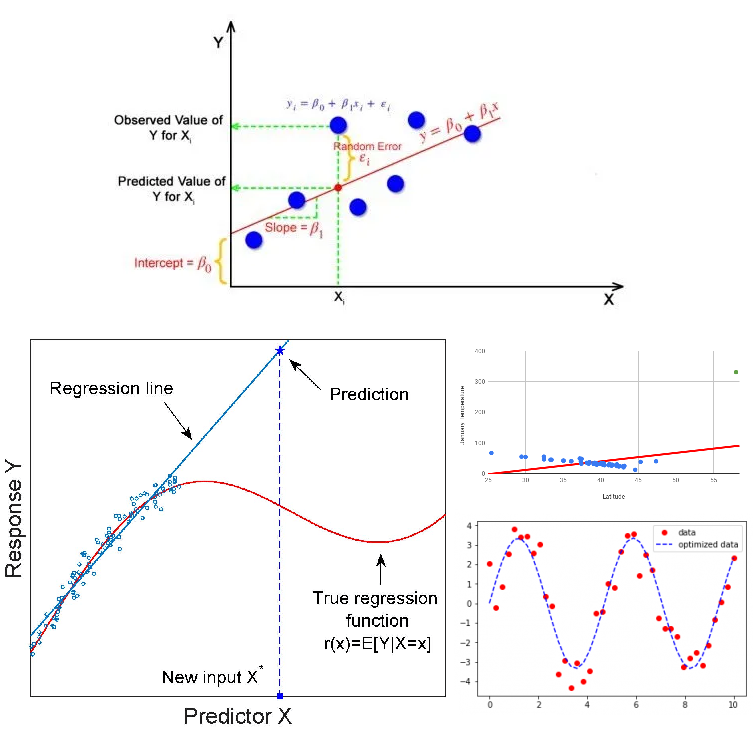
\includegraphics[angle=0, width=.61225\textwidth] {regression.png}
\end{center}
\end{figure}
\end{itemize}
\end{document}
